\section{Study Settings}

Before the conception of droidXP, there were studies that provided valuable information about the comparison between test generation tools \cite{bao2018mining}\cite{hao2014puma}. This data was required to measure the benchmark droidXP's performance and precision. Particularly, L Bao et al. \cite{bao2018mining} had provided an important comparative study between five test generation tools in finding malware using mining sandboxes techniques, and that inspired our study settings. His first experiment used a small set of apps (10 pairs B/M) to be run for different periods of time to compare how much time the tools needed to achieve the maximum coverage possible and to identify the sensitive APIs accessed. This study showed that the coverage and accuracy of the testing tool have a negative correlation. That is, improving the performance of code coverage might not directly contribute to the performance of detecting malware. The second experiment used a set of 102 pairs of apps that were executed for just one minute. The goal of this experiment was to compare a bigger number of apps and the number of sensitive APIs accessed by each tool in a small time. However, this study did not focus on the possible interference of the DroidFax \cite{cai2017droidfax} tool on the benchmark results. The benchmark uses DroidFax to analyze Android apps during execution, but this tool also performs a static analysis of the apps.

The first empirical study had shown useful aspects of the tools while being executed by the benchmark droidXP. To replicate the previous studies, we choice a subset of pairs (B/M), based on the set of pairs presented by L Bao et al. The addition of Humanoid and the fake tools, "Joke", in the comparison brought newer techniques that explored Android apps better.

Hence, the main goal of this research work is
to understand the influence of the static analysis, which is performed by DroidFax, in the benchmark execution. To achieve this general goal, we answer the following research questions. 


\begin{enumerate}[(RQ1)]
\item What is the effective performance of each tool in terms of the number of detected malware ?
\item What benefits of using a hybrid approach, which combines static and dynamic analysis, for mining sandboxes ?
\item What is the impact of DroidFax’s static analysis on benchmark results ?
\end{enumerate}

In the first experiment, we executed the benchmark considering 98 pairs of apps for 3 minutes. At this time, we used a new option of the benchmark that disables the static analysis performed by DroidFax. So, we used this experiment to answer the first research questions (RQ1). In the second experiment, we executed all apps with a fake tool called “Joke”, which does not do anything during the benchmark execution, to compute the results without the dynamic analysis influence. With these results, we can answer the last two research question (RQ2 and RQ3).

\subsection{Settings for RQ1}

To assess the effectiveness of mining sandboxes created by each test case generation tools, we run these tools in benign apps and, based on resources sensitives access in this execution, we build their sandbox. Based on this sandbox, we investigate the capacity of detect malicious behaviors in the corresponding malign app. (Figure  \ref{fig:setup}) show all this experimental setup.


\subsection{Settings for RQ2 and RQ3}


\begin{figure*}[h!]
  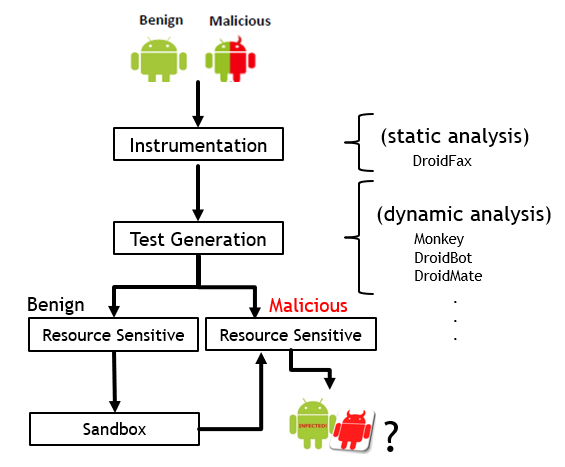
\includegraphics[width=0.5\textwidth]{images/setup.png}
  \label{Experiment setup}
  \caption{Experiment setup}
  \label{fig:setup}
\end{figure*}


\subsection{Experiment motivation}

As described 
